\documentclass[class=report, crop=false, 12pt,a4paper]{standalone}
\usepackage{enumitem}
\usepackage{multicol}
\usepackage{graphicx}
\usepackage{float}
\usepackage{amsmath}
\usepackage{amssymb}
\usepackage{mathtools}
\usepackage{siunitx}
\usepackage{commath}
\usepackage{array}
\usepackage{natbib}
\usepackage[a4paper,width=150mm,top=25mm,bottom=25mm]{geometry}
\setlength{\parindent}{0pt}
\begin{document}
\section{Statically Indeterminate Beams}
\begin{center}
  30/10/2020
\end{center}
So far, we have analysed statically-determinate beams. These are characterised by only \textbf{two unknown support reactions}, that can be determined from the force and moment equilibrium equations. \\\\
If the supports produce \textbf{three or more unknown reactions}, the beam is \textbf{statically indeterminate}.
\begin{figure}[H]
  \centering
  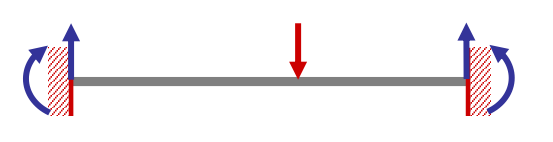
\includegraphics[width = 0.8 \textwidth]{../img/beam11.PNG}
\end{figure}
The analysis of statically indeterminate structures requires the calculation of displacements to find a sufficient number of equations to solve for all unknown reactions. \\\\
The double integration method or the Macaulay’s method can be used to find the support reactions and the solution in statically indeterminate problems.
\subsubsection{Example: Propped Cantilever with Uniformly Distributed Load (Double Integration Method)}
\begin{figure}[H]
  \centering
  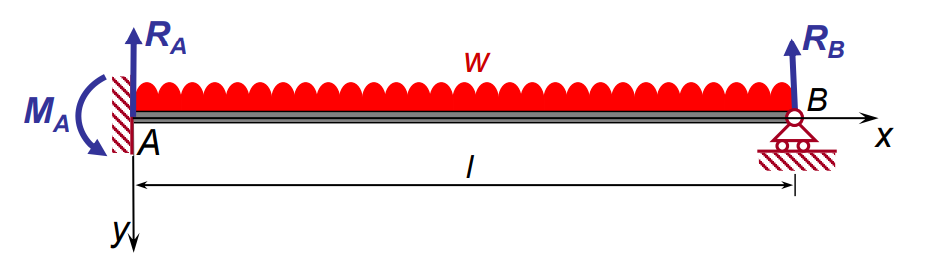
\includegraphics[width = 0.9 \textwidth]{../img/beam12.PNG}
\end{figure}
The equilibrium equations:
\begin{gather}
  R_A-wl+R_B = 0 \\
  R_Al-M_A-\frac{1}{2}wl^2 = 0
\end{gather}
Moment at the point distance $x$ away from the left end:
\begin{gather}
  M(x) = -M_A-\frac{1}{2}wx^2+R_Ax
\end{gather}
Integrating the moment equation:
\begin{gather}
  \theta(x) = \frac{\dif y}{\dif x} = -\frac{1}{EI}\int\left(-M_A-\frac{1}{2}wx^2+R_Ax\right)\dif x \\
  = -\frac{1}{EI}\left(-M_Ax-\frac{1}{6}wx^3+\frac{1}{2}R_Ax^2\right) + \theta_0
\end{gather}
Boundary Condition: $\theta(0) = 0 \longrightarrow \theta_0 = 0$
\begin{gather}
  \therefore \theta(x) = -\frac{1}{EI}\left(-M_Ax-\frac{1}{6}wx^3+\frac{1}{2}R_Ax^2\right)
\end{gather}
Integrating further:
\begin{gather}
  y(x) = -\frac{1}{EI}\int\left(-M_Ax-\frac{1}{6}wx^3+\frac{1}{2}R_Ax^2\right)\dif x \\
  = -\frac{1}{EI}\left(-\frac{1}{2}M_Ax^2-\frac{1}{24}wx^4+\frac{1}{6}R_Ax^3\right) + y_0
\end{gather}
Boundary Condition: $y(0) = 0 \longrightarrow y_0 = 0$
\begin{gather}
  \therefore y(x) = -\frac{1}{EI}\left(-\frac{1}{2}M_Ax^2-\frac{1}{24}wx^4+\frac{1}{6}R_Ax^3\right)
\end{gather}
Applying another boundary condition $y(l) = 0$ (to consider the other end of the beam):
\begin{gather}
  y(l) = -\frac{1}{EI}\left(-\frac{1}{2}M_Al^2-\frac{1}{24}wl^4+\frac{1}{6}R_Al^3\right) = 0 \\
  \longrightarrow \frac{1}{2}M_Al^2+\frac{1}{24}wl^4-\frac{1}{6}R_Al^3 = 0 \\
  \longrightarrow 12M_A + wl^2 - 4R_Al = 0
  \label{doubleintegration}
\end{gather}
The $R_A$, $R_B$, and $M_A$ are still \textbf{unknowns} at this point. Combining the equilibrium conditions with the double integration (equation (\ref{doubleintegration})):
\begin{gather}
  R_A-wl+R_B = 0 \\
  R_Al-M_A-\frac{1}{2}wl^2 = 0 \\
  4R_Al-12M_A-wl^2 = 0 
\end{gather}
Solving for the above system of equations yields:
\begin{gather}
  R_A = \frac{5}{8}wl \\
  R_B = \frac{3}{8}wl \\
  M_A = \frac{wl^2}{8}
\end{gather}
Using these values in all previous equations, all quantities can be determined.
\begin{figure}[H]
  \centering
  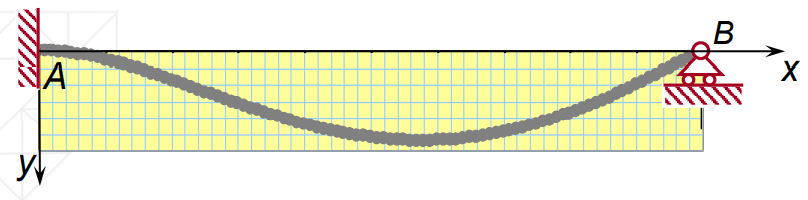
\includegraphics[width = 0.9 \textwidth]{../img/graph1.PNG}
\end{figure}
\subsubsection{Example: Fixed Beam with Concentrated Load (Macaulay's Method)}
\begin{figure}[H]
  \centering
  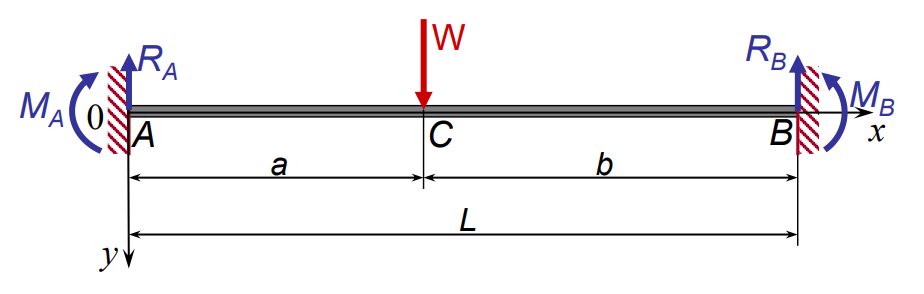
\includegraphics[width = 0.9 \textwidth]{../img/beam13.PNG}
\end{figure}
The equilibrium conditions:
\begin{gather}
  R_A-W+R_B = 0 \\
  M_A-Wb+R_AL-M_B = 0
\end{gather}
Moment at the point distance $x$ away from the left end:
\begin{gather}
  M(x) = M_A+R_Ax-W\langle x-a \rangle 
\end{gather}
Integrating the moment equation:
\begin{gather}
  \theta(x) = \frac{\dif y}{\dif x} = -\frac{1}{EI}\int\left(M_A+R_Ax-W\langle x-a \rangle\right) \dif x \\
  = -\frac{1}{EI}\left(M_Ax+\frac{1}{2}R_Ax^2-\frac{1}{2}W\langle x-a\rangle^2\right) + \theta_0
\end{gather}
Boundary Condition: $\theta(0) = 0 \longrightarrow \theta_0 = 0$
\begin{gather}
  \therefore \theta(x) = -\frac{1}{EI}\left(M_Ax+\frac{1}{2}R_Ax^2-\frac{1}{2}W\langle x-a\rangle^2\right)
\end{gather}
Integrating further:
\begin{gather}
  y(x) = -\frac{1}{EI}\int\left(M_Ax+\frac{1}{2}R_Ax^2-\frac{1}{2}W\langle x-a\rangle^2\right) \dif x \\
  = -\frac{1}{EI}\left(\frac{1}{2}M_Ax^2+\frac{1}{6}R_Ax^3-\frac{1}{6}W\langle x-a \rangle^3\right) + y_0
\end{gather}
Boundary Condition: $y(0) = 0 \longrightarrow y_0 = 0$
\begin{gather}
  \therefore y(x) = -\frac{1}{EI}\left(\frac{1}{2}M_Ax^2+\frac{1}{6}R_Ax^3-\frac{1}{6}W\langle x-a \rangle^3\right)
\end{gather}
Applying other boundary conditions $\theta(L) = 0$, $y(L) = 0$ (to consider the other end of the beam):
\begin{gather}
  \theta(L) = -\frac{1}{EI}\left(M_AL+\frac{1}{2}R_AL^2-\frac{1}{2}W(L-a)^2\right) = 0 \\
  y(L) = -\frac{1}{EI}\left(\frac{1}{2}M_AL^2+\frac{1}{6}R_AL^3-\frac{1}{6}W(L-a)^3\right) = 0
\end{gather}
\begin{gather}
  \text{Overall:}
  \begin{cases}
    R_A-W+R_B = 0 \\
    M_A-Wb+R_AL-M_B = 0 \\
    2M_AL+R_AL^2-W(L-a)^2 = 2M_AL+R_AL^2-Wb^2 = 0 \\
    3M_AL^2+R_AL^3-W(L-a)^3 = 3M_AL^2+R_AL^3-Wb^3 = 0
  \end{cases}
\end{gather}
The $R_A$, $R_B$, $M_A$, and $M_B$ are the 4 \textbf{unknowns} with 4 equations. Hence, they can be solved:
\begin{gather}
  R_A = \frac{Wb^2}{L^3}(3a+b) \\
  M_A = -\frac{Wab^2}{L^2} \\
  R_B = \frac{Wa^2}{L^3}(3b+a) \\
  M_B = -\frac{Wa^2b}{L^2}
\end{gather}
The equation of deflection:
\begin{gather}
  y = -\frac{W}{2EI}\left[\frac{b^2(3a+b)x^3}{3L^3}-\frac{ab^2x^2}{L^2}-\frac{\langle x-a \rangle^3}{3}\right] \\
  y(a) = \frac{Wa^3b^3}{3EIL^3}
\end{gather}
\begin{figure}[H]
  \centering
  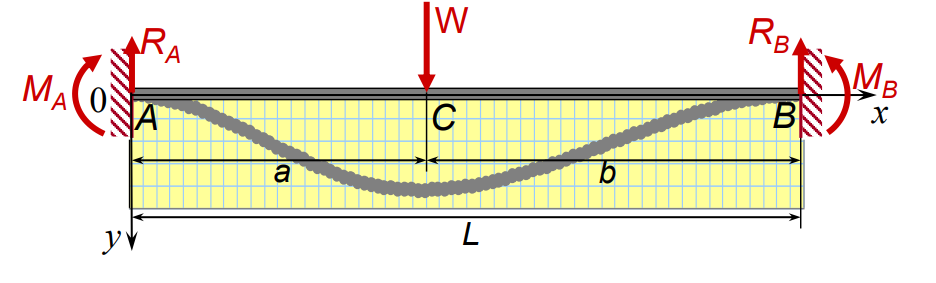
\includegraphics[width = 0.9 \textwidth]{../img/graph2.PNG}
\end{figure}
\begin{figure}[H]
  \centering
  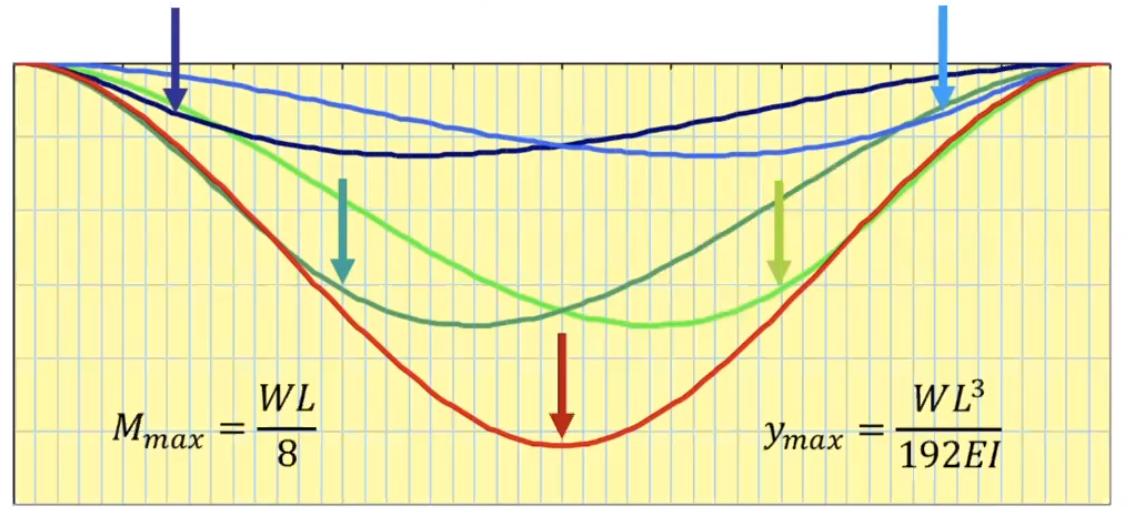
\includegraphics[width = 0.8 \textwidth]{../img/graph3.PNG}
  \caption{Depending on the loading, the profile of the deflection will be different. Maximum diflection occurs when $a=b=\frac{L}{2}$}
\end{figure}
Statically indeterminate structures produce \textbf{lower displacement and stress levels}, resulting in savings in material.
\textbf{Failure} of a member in a statically determinate structure \textbf{leads to collapse}. In case of failure of a member, statically indeterminate structures can find \textbf{alternative load paths}, at least temporarily.
\end{document}